\section{LuckyPatcher} \label{section:luckypatcher-explain}
LuckyPatcher is described as "[...] a great Android tool to remove ads, modify apps permissions, backup and restore apps, bypass premium applications license verification, and more" on the official website \cite{luckyPatcherOfficial}.
It is written by ChelpuS and currently on version is 6.0.4 (on 02/17/2016).
Since applications are stored that the user cannot access them (see subsection~\ref{subsection:android-copyroot}), root is neccesary to use the application.
In addition, busybox, an application which provides standard UNIX tools for Android\cite{busyboxApp}, is required as well.
\newline
LuckyPatcher offeres the removing of the licensing in premium apps to crack their \gls{drm}, to remove inapp ads, change and restrict permissions and activities as well as to create modified after applying one of the feature above on the original \gls{apk}s \cite{luckyPatcherOfficial}.
\newline
The application requires, besides of rooting, no technical knowledge to handle and offeres automatic cracking for non professionals.
This combination makes it a popular and an effective tool with a high damage potential. \cite{munteanLicense}
\newline
This thesis focuses on how LuckyPatcher is bypassing the license verification mechanism of applications.
The goal of circumventing the license check is to make the pirated application to work as it would have been legally aquired in the store.
As described in section~\ref{section:lvl}, the license verifications are implemented as client-server connection.
The app gathers the information, sends it to the server, which checks the verifies the given information, and replies the result to the client.
Since the server is not accessible, an man-in-the middle attack or spoofing would be an obvious options to break the license verification mechanism.
The execution of these is very difficult since breaking encryption in general is hard to carry out \cite{munteanLicense}.
This is the reason why LuckyPatcher is taking a different path by modifying the application itself. This will be analysed in detail in the following chapters after explaining the general usage.
\newline
\begin{figure}[h]
    \centering
    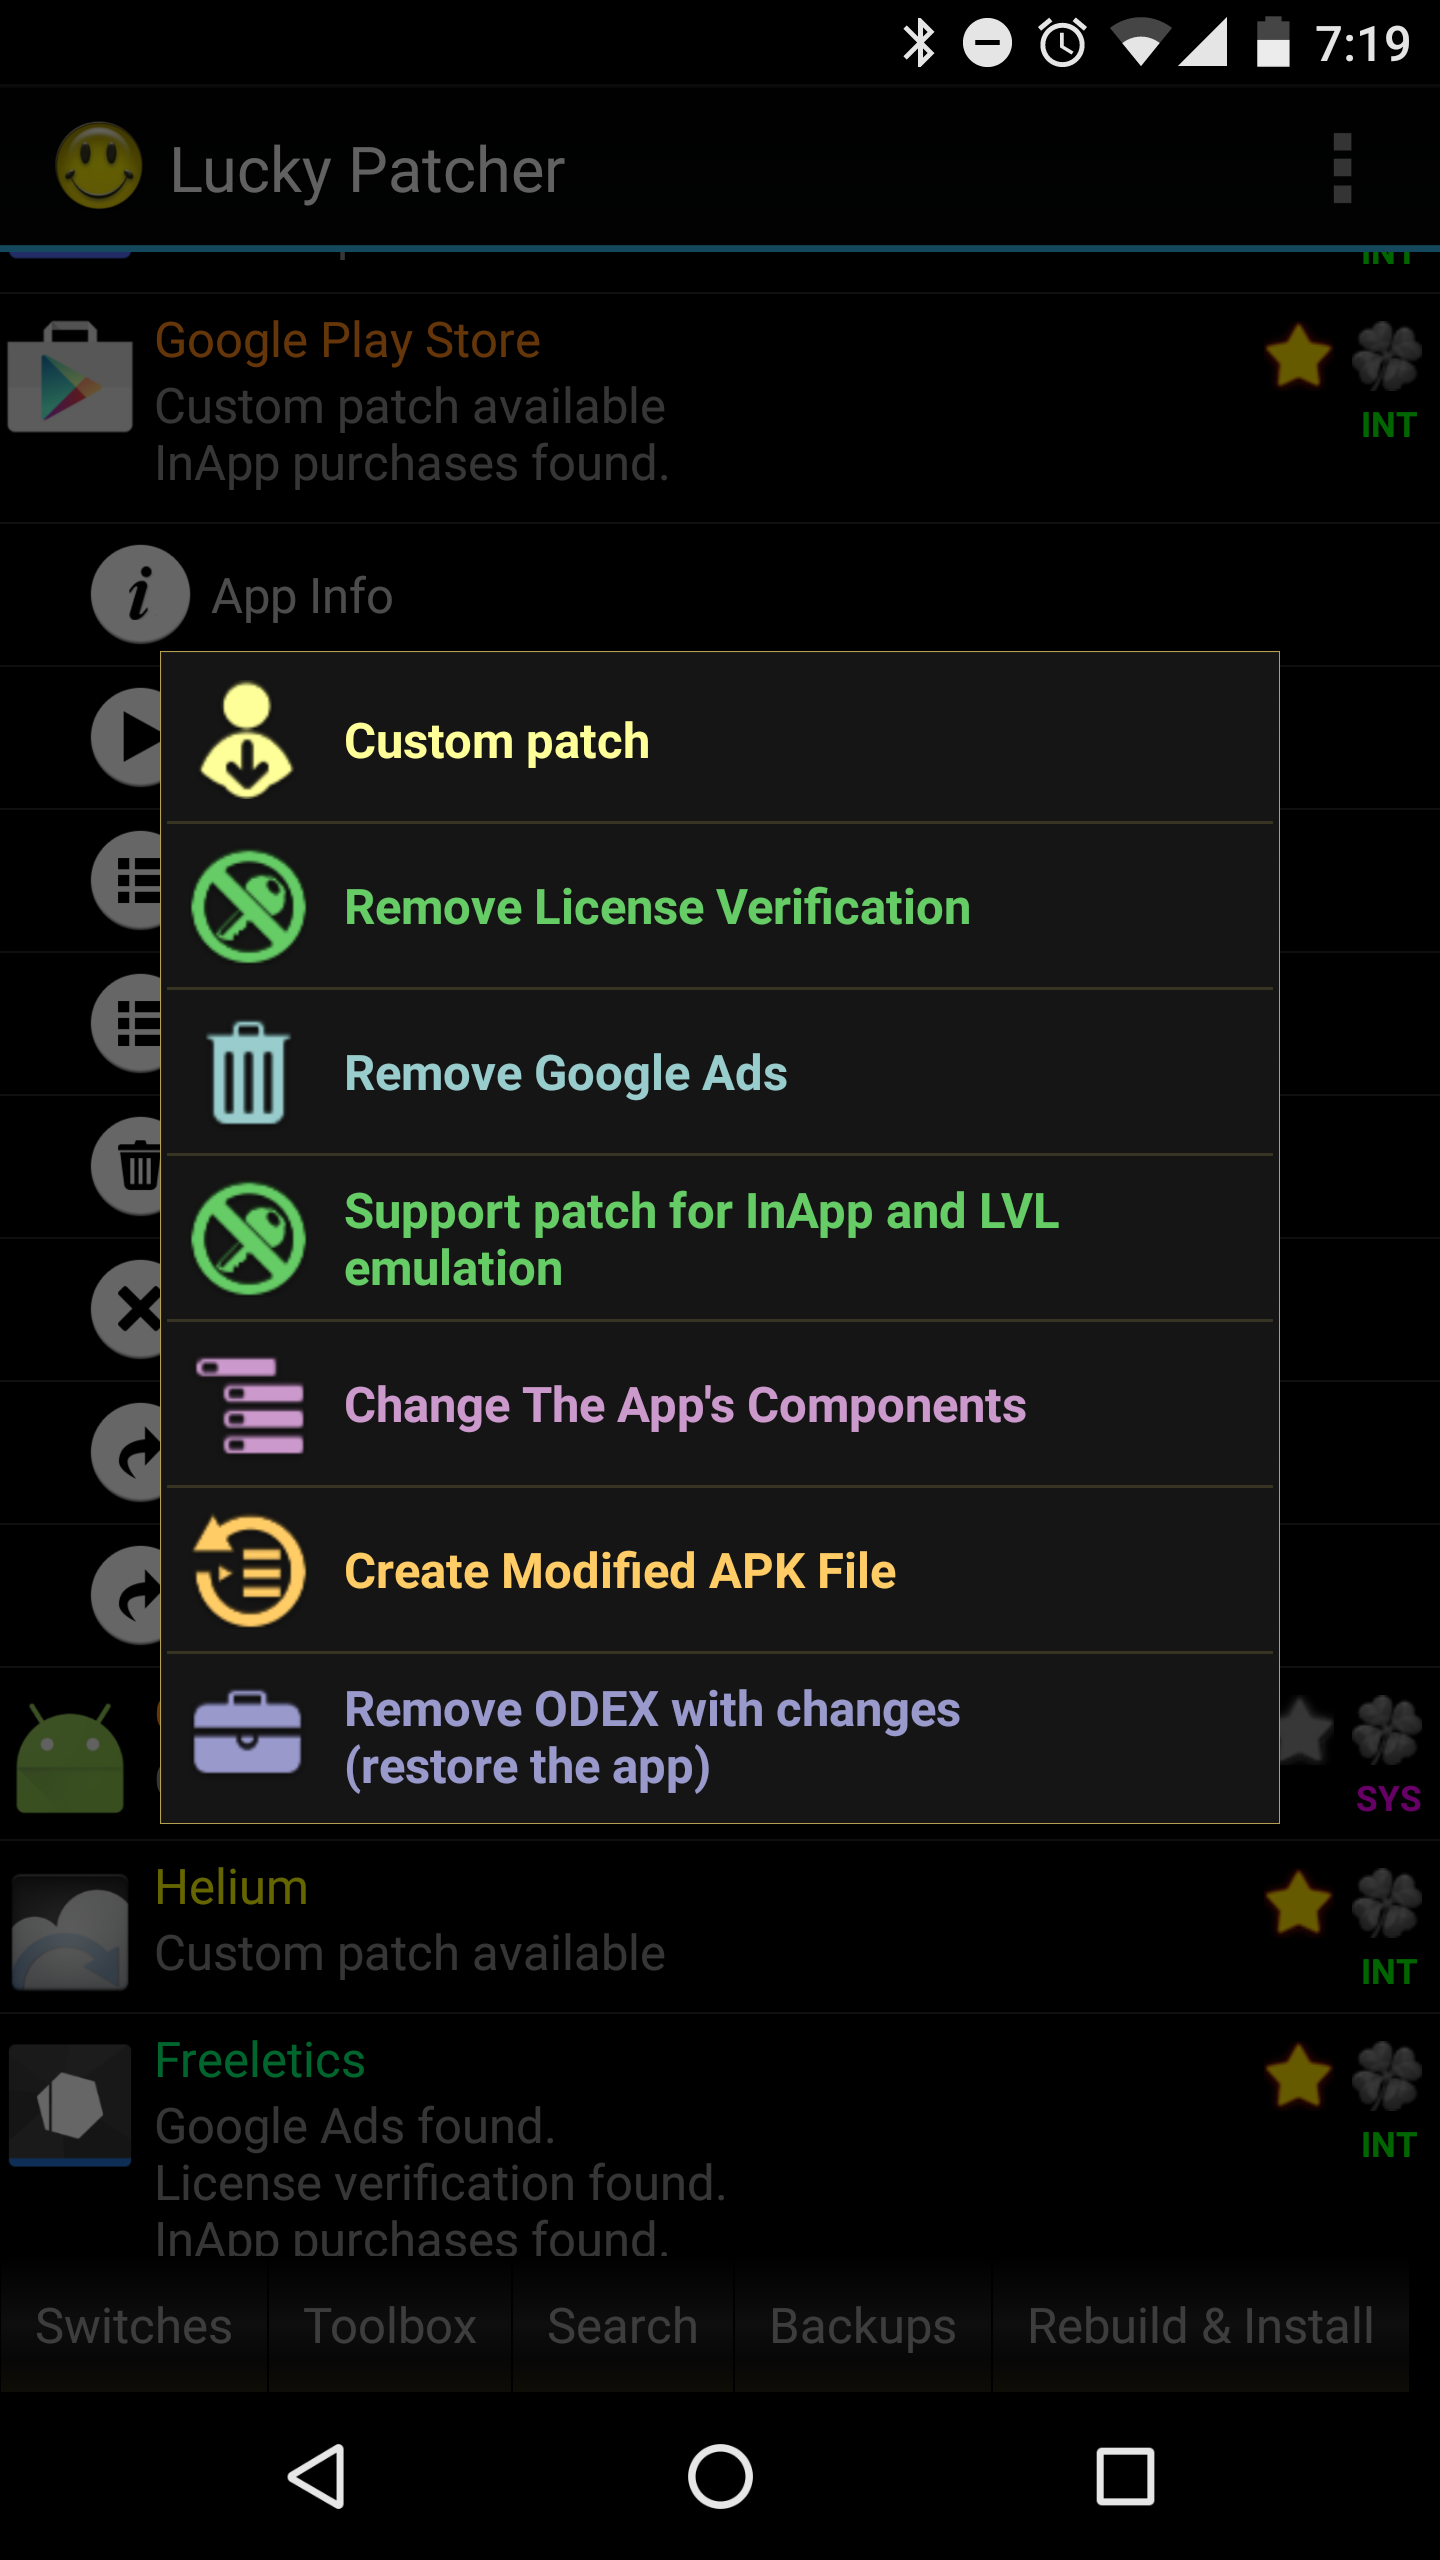
\includegraphics[width=0.3\textwidth]{data/luckyFeatures.png}
    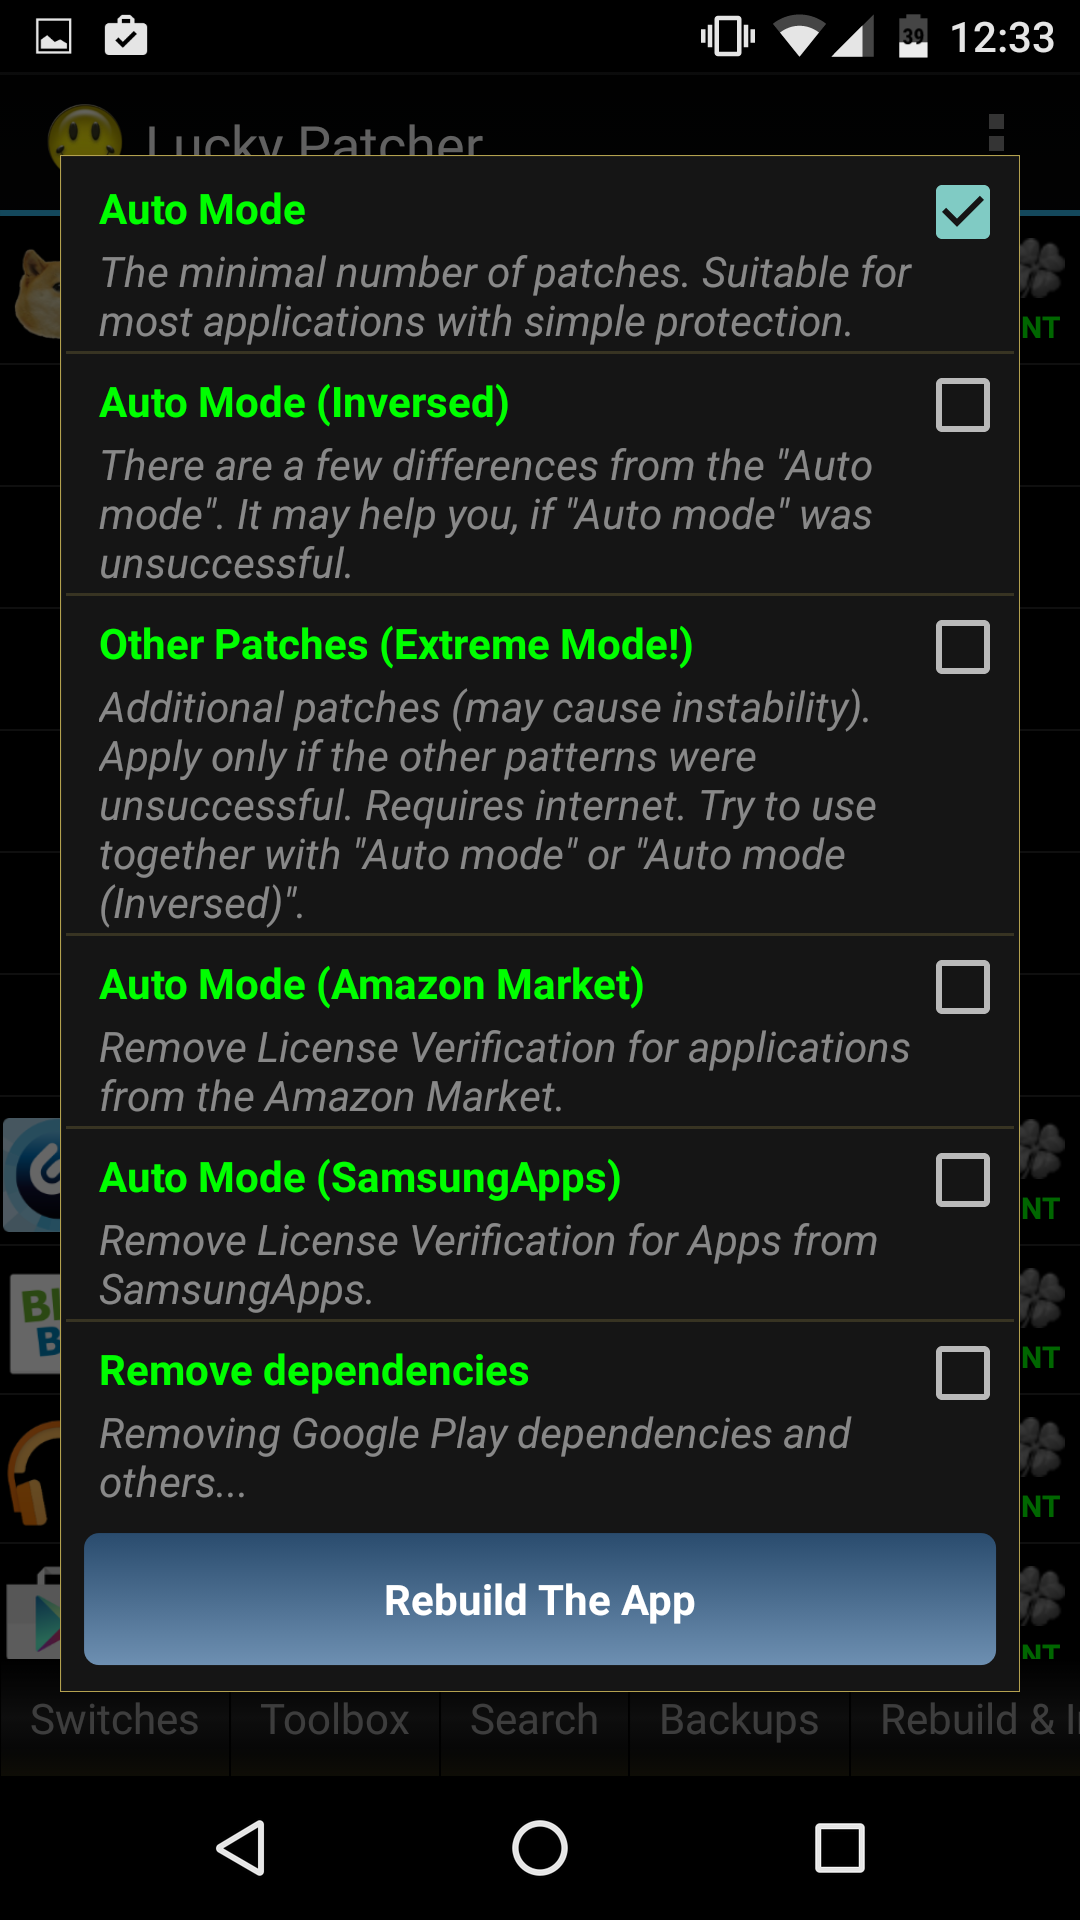
\includegraphics[width=0.3\textwidth]{data/luckyModi.png}
    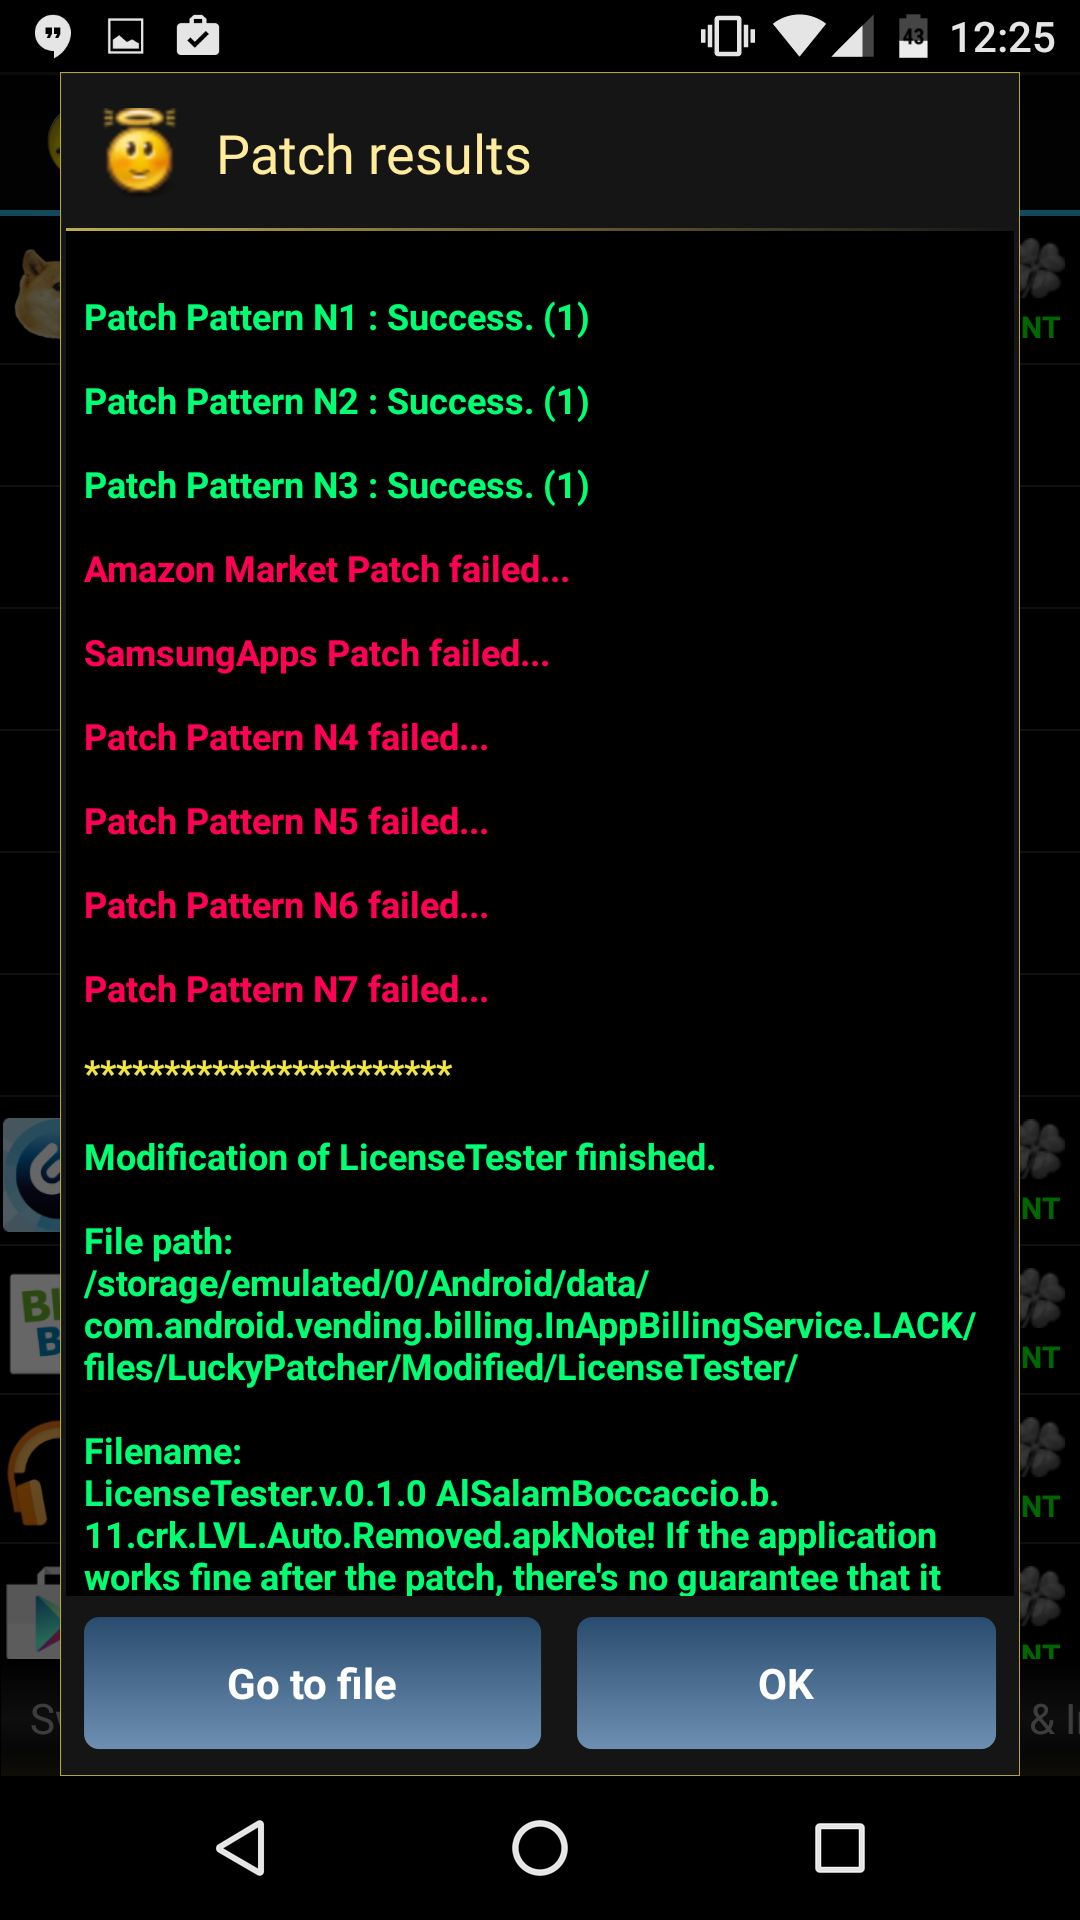
\includegraphics[width=0.3\textwidth]{data/luckyPatching.png}
    \caption{c}{Left to right: Features offered LuckyPatcher, modes to crack license verification and the result after patching}
    \label{fig:luckyScreen}
\end{figure}

Using LuckyPatcher is fairly simple.
The application can be downloaded from the official website \cite{luckyPatcherOfficial} as an \gls{apk} and installed on the device.
In order to have the features availablem, the device has to be rooted.
On startup, all installed applications are shown in a list.
Below their name an information about what patches can be applied is shown.
When a the application is selected, a submenu offeres actions like to get information about the app or to run it to name a few.
The action required to modify the application is the menu of patches which offeres the features described above and can be seen on figure~\ref{fig:luckyScreen} on the left.
In this menu there are two choices to achieve the license verification.
In case the crack should be applied directly on the device, the license verification removing can be chosen, else LuckyPatcher creates an modified apk, which can include the modified license verification mechanism.
When the output of choice is selected, different modes can be selected.
The description of what they are doing can be seen in figure~\ref{fig:luckyScreen} in the middle and is rather short.
A closer analysis of the different modes is done and presented in section~\ref{section:luckypatcher-modi}.
After chosing the mode of choice the actual patching is done and the result are shown as seen in figure~\ref{fig:luckyScreen} on the right.
The different patching patterns will be analysed and explained in section~\ref{section:luckypatcher-patterns}.
LuckyPatcher does not offer a 100\% warranty that the result is working and all license verification related restrictions are removed.
\newline
For this thesis LuckyPatcher is analysed in two different ways.
On the one hand the source code reengineered and the functionality of the reversed code is inspected.
On the other hand the cracking tool is applied to different applications and the result was compared to the original in order to see how LuckyPatcher is applying patches.

%soll ich schreiben welche apps und approvements anhängen? pattern results anhängen?

%%update auf neuere version?
